\documentclass{beamer}%[handout]
\usetheme{Boadilla}%Berlin}
\usepackage[T1]{fontenc}
\usepackage[utf8]{inputenc}
\usepackage{lmodern}
\usepackage{amsmath}
\usepackage{amsthm}
\usepackage{amsopn}
%\usepackage{cite}
\usepackage{pdflscape}
\usepackage{afterpage}
\usepackage{changepage}
\usepackage{caption}
\usepackage{colortbl}
\usepackage{adjustbox}
\usepackage{hyperref}
\usepackage{caption}
\usepackage{subcaption}

%\usepackage[style=authoryear]{biblatex}
%\bibliography{revbibl}
\usepackage{graphicx}
\usepackage{cite}
\usepackage{apacite}
\setlength{\arrayrulewidth}{1pt}
\usepackage{tikz}
    \usetikzlibrary{positioning}
    \usetikzlibrary{decorations.pathreplacing}
    \usetikzlibrary{fadings}
    \usetikzlibrary{matrix}

\tikzset{basic/.style={draw,fill=blue!20,text width=1em,text badly centered}}
\tikzset{input/.style={basic,circle}}
\tikzset{weights/.style={basic,rectangle}}
\tikzset{functions/.style={basic,circle,fill=blue!10}}
\tikzset{hidden/.style={draw,shape=circle,fill=blue!30,minimum size=1.15cm}}
\tikzset{output/.style={draw,shape=circle,fill=red!20,minimum size=1.15cm}}

\newcommand\blfootnote[1]{%
  \begingroup
  \renewcommand\thefootnote{}\footnote{#1}%
  \addtocounter{footnote}{-1}%
  \endgroup
}

\makeatother
\setbeamertemplate{footline}
{
  \leavevmode%
  \hbox{%
  \begin{beamercolorbox}[wd=.2\paperwidth,ht=2.25ex,dp=1ex,center]{author in head/foot}%
    \usebeamerfont{author in head/foot}\insertshortauthor
  \end{beamercolorbox}%
  \begin{beamercolorbox}[wd=.8\paperwidth,ht=2.25ex,dp=1ex,center]{title in head/foot}%
    \usebeamerfont{title in head/foot}
    \insertshorttitle{}\hspace*{12ex}
    \insertframenumber/\inserttotalframenumber%\hspace*{1ex}
  \end{beamercolorbox}
  }%
  \vskip0pt%
}
\makeatletter
\setbeamertemplate{navigation symbols}{}

\theoremstyle{definition}
\newtheorem*{proposition}{Proposition}

\theoremstyle{definition}
\newtheorem*{enboxed}{}

\theoremstyle{example}
\newtheorem*{code_ex}{Code Example}

\theoremstyle{example}
\newtheorem*{remark}{Remark}

\newcommand{\srcsize}{\@setfontsize{\srcsize}{5pt}{5pt}}

\begin{document}
\title{Simple Neural Networks in  PyTorch vs Tensorflow}
\subtitle{Fast intro for beginners}


\author{Krzysztof Podlaski}

\date{\tiny Seminarium\\
Katedry Systemów Inteligentnych\\
Uniwersytet Łódzki\\
31 Marca 2023}

\begin{frame}
\titlepage
\end{frame}


\section{Neural network libraries in python}
\begin{frame}
W have two main Machine Learning tools in python:
\begin{itemize}
\item PyTorch -- library for advanced programmers, more control, but also more details and coding.
\item Tensorflow -- much nicer library for the start.
\end{itemize}

Both support GPU computing, PyTorch is said to do better in distributed GPU systems.
\end{frame}
\begin{frame}[fragile]{Dense network}

Dense networks are the most classical architectures. MLP -- Multilayer Perceptron.

We have set of neurons, each have inputs and weights, sums them up, add bias and activation function.

\begin{equation*}
  y = f(\sum_i x_iw_i+b)
\end{equation*}

\begin{figure}
\begin{subfigure}[b]{0.3\textwidth}
\centering
\resizebox{\textwidth}{!}{
% source https://tex.stackexchange.com/questions/104334/tikz-diagram-of-a-perceptron
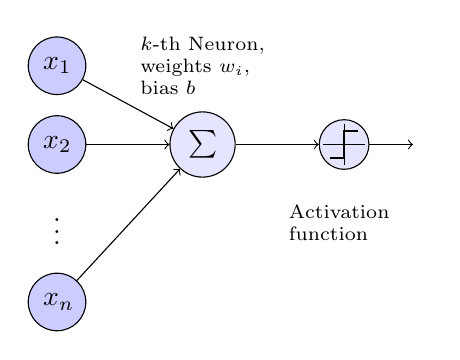
\begin{tikzpicture}
        \node[functions] (center) {};
        \node[functions,left=3em of center] (left) {$\sum$};
            \path[draw,->] (left) -- (center);
        \node[below of=center,font=\scriptsize,text width=4em] {Activation function};
        \node[above of=left,font=\scriptsize,text width=4.5em] {$k$-th Neuron,\\weights $w_{i}$,\\bias $b$};
        \draw[thick] (0.5em,0.5em) -- (0,0.5em) -- (0,-0.5em) -- (-0.5em,-0.5em);
        \draw (0em,0.75em) -- (0em,-0.75em);
        \draw (0.75em,0em) -- (-0.75em,0em);
        \node[right of=center] (right) {};
            \path[draw,->] (center) -- (right);
        
        \node[input,left=3em of left] (2) {$x_2$} ;
            \path[draw,->] (2) -- (left);
        \node[below of=2] (dots) {$\vdots$} ;
        \node[input,below of=dots] (n) {$x_n$} ;
            \path[draw,->] (n) -- (left);
        \node[input,above of=2] (1) {$x_1$} ;
            \path[draw,->] (1) -- (left);
        
    \end{tikzpicture}

}
\end{subfigure}
\hfill
\begin{subfigure}[b]{0.6\textwidth}
\resizebox{\textwidth}{!}{
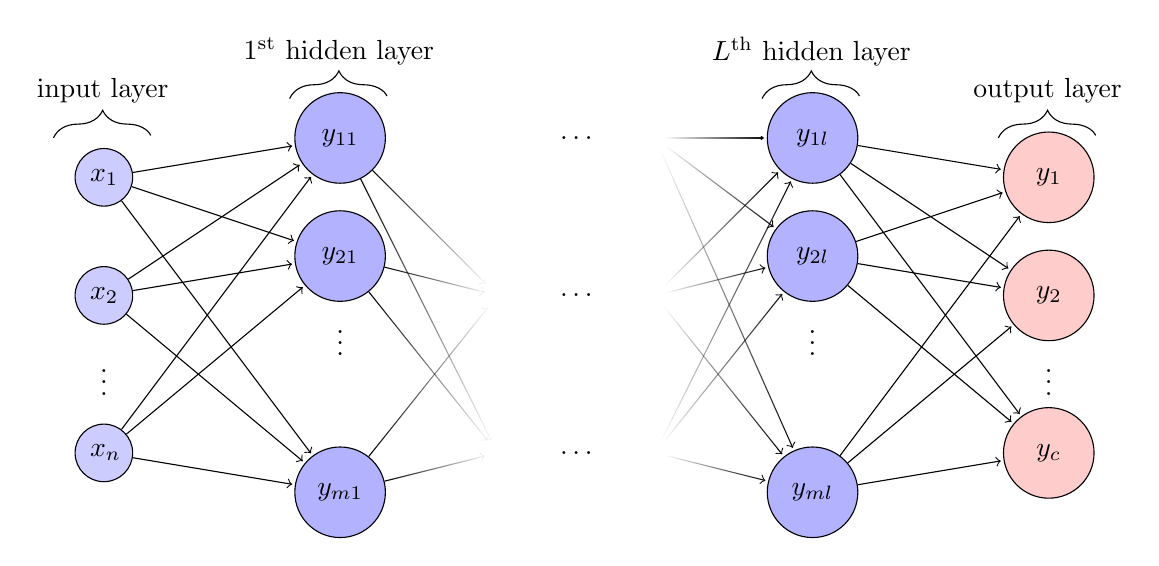
\begin{tikzpicture}[shorten >=1pt]
		\tikzstyle{unit}=[draw,shape=circle,minimum size=1.15cm]
		%\tikzstyle{hidden}=[draw,shape=circle,fill=black!25,minimum size=1.15cm]
		%\tikzstyle{hidden}=[draw,shape=circle,minimum size=1.15cm]

		\node[input](x0) at (0,3.5){$x_1$};
		\node[input](x1) at (0,2){$x_2$};
		\node at (0,1){\vdots};
		\node[input](xd) at (0,0){$x_n$};

		\node[hidden](h10) at (3,4){$y_{11}$};
		\node[hidden](h11) at (3,2.5){$y_{21}$};
		\node at (3,1.5){\vdots};
		\node[hidden](h1m) at (3,-0.5){$y_{m1}$};

		\node(h22) at (5,0){};
		\node(h21) at (5,2){};
		\node(h20) at (5,4){};
		
		\node(d3) at (6,0){$\ldots$};
		\node(d2) at (6,2){$\ldots$};
		\node(d1) at (6,4){$\ldots$};

		\node(hL12) at (7,0){};
		\node(hL11) at (7,2){};
		\node(hL10) at (7,4){};
		
		\node[hidden](hL0) at (9,4){$y_{1l}$};
		\node[hidden](hL1) at (9,2.5){$y_{2l}$};
		\node at (9,1.5){\vdots};
		\node[hidden](hLm) at (9,-0.5){$y_{ml}$};

		\node[output](y1) at (12,3.5){$y_1$};
		\node[output](y2) at (12,2){$y_2$};
		\node at (12,1){\vdots};	
		\node[output](yc) at (12,0){$y_c$};

        \draw[->] (x0) -- (h10);
		\draw[->] (x0) -- (h11);
		\draw[->] (x0) -- (h1m);

        \draw[->] (x1) -- (h10);
		\draw[->] (x1) -- (h11);
		\draw[->] (x1) -- (h1m);
        
        \draw[->] (xd) -- (h10);
		\draw[->] (xd) -- (h11);
		\draw[->] (xd) -- (h1m);


		\draw[->] (hL0) -- (y1);
		\draw[->] (hL0) -- (yc);
		\draw[->] (hL0) -- (y2);

		\draw[->] (hL1) -- (y1);
		\draw[->] (hL1) -- (yc);
		\draw[->] (hL1) -- (y2);

		\draw[->] (hLm) -- (y1);
		\draw[->] (hLm) -- (y2);
		\draw[->] (hLm) -- (yc);

		\draw[->,path fading=east] (h10) -- (h21);
		\draw[->,path fading=east] (h10) -- (h22);
		
		\draw[->,path fading=east] (h11) -- (h21);
		\draw[->,path fading=east] (h11) -- (h22);
		
		\draw[->,path fading=east] (h1m) -- (h21);
		\draw[->,path fading=east] (h1m) -- (h22);
		
        \draw[->,path fading=west] (hL10) -- (hL0);
		\draw[->,path fading=west] (hL11) -- (hL0);
		\draw[->,path fading=west] (hL12) -- (hL0);

		\draw[->,path fading=west] (hL10) -- (hL1);
		\draw[->,path fading=west] (hL11) -- (hL1);
		\draw[->,path fading=west] (hL12) -- (hL1);
		
		\draw[->,path fading=west] (hL10) -- (hLm);
		\draw[->,path fading=west] (hL11) -- (hLm);
		\draw[->,path fading=west] (hL12) -- (hLm);
		
		\draw [decorate,decoration={brace,amplitude=10pt},xshift=-4pt,yshift=0pt] (-0.5,4) -- (0.75,4) node [black,midway,yshift=+0.6cm]{input layer};
		\draw [decorate,decoration={brace,amplitude=10pt},xshift=-4pt,yshift=0pt] (2.5,4.5) -- (3.75,4.5) node [black,midway,yshift=+0.6cm]{$1^{\text{st}}$ hidden layer};
		\draw [decorate,decoration={brace,amplitude=10pt},xshift=-4pt,yshift=0pt] (8.5,4.5) -- (9.75,4.5) node [black,midway,yshift=+0.6cm]{$L^{\text{th}}$ hidden layer};
		\draw [decorate,decoration={brace,amplitude=10pt},xshift=-4pt,yshift=0pt] (11.5,4) -- (12.75,4) node [black,midway,yshift=+0.6cm]{output layer};
	\end{tikzpicture}
}
\end{subfigure}\blfootnote{\tiny pictures based on \url{https://tex.stackexchange.com/questions/104334/tikz-diagram-of-a-perceptron} and \url{https://tikz.net/neural_networks/}}
\end{figure}

\end{frame}

\begin{frame}{Dataset -- MNIST}
\begin{itemize}
\item contains images of digits
\item each image 28x28 gray scale
\item all have assigned labels
\item incorporated with PyTorch and Tensorflow
\end{itemize}
\begin{figure}
\centering
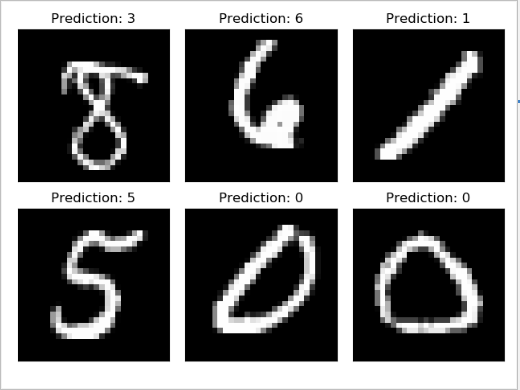
\includegraphics[width=.6\textwidth]{images/mnist.png}
\end{figure}
\end{frame}

\begin{frame}{Basic info about implementation}
\begin{itemize}
  \item All codes are on github: \url{https://github.com/kpodlaski/NeuralNetworksIntro}
  \item Dense network are in directory: examples $\rightarrow$ DenseNetwork
  \item Tensorflow is in: examples $\rightarrow$ DenseNetwork $\rightarrow$ tensorflow
  \item PyYorch is in: examples $\rightarrow$ DenseNetwork $\rightarrow$ pytorch \\and common $\rightarrow$ pytorch
  \item Task: digit recognition (classification)
\end{itemize}
\end{frame}


\begin{frame}{Dense network architecture (MLP)}
Implemented in both libraries
\begin{itemize}
  \item input layer -- 794 signals ($28\times28$)
  \item 1st layer -- 320 neurons tanh activation
  \item 2nd layer -- 240 neurons sigmoid activation
  \item 3rd layer -- 120 neurons relu activation
  \item out layer -- 10 neurons softmax activation
\end{itemize}
\end{frame}


\begin{frame}[fragile]{Convolution Layer}

\begin{equation}
(I*K)_m,n = \sum_{i}\sum_{k}I_{j,k}K_{m-j, n-k}
\end{equation}

\begin{figure}
  \centering
  % Convolution operator.
% Adapted from https://github.com/PetarV-/TikZ/tree/master/2D%20Convolution

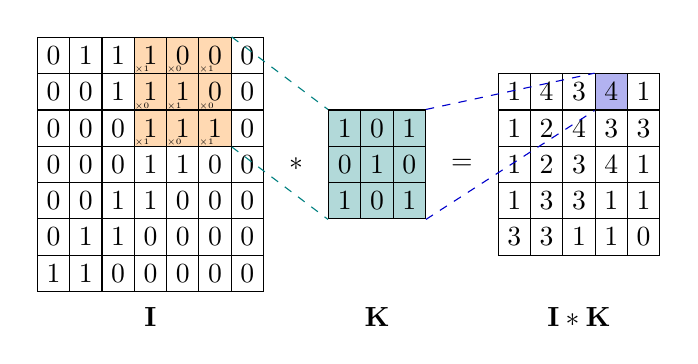
\begin{tikzpicture}[
    2d-arr/.style={matrix of nodes, row sep=-\pgflinewidth, column sep=-\pgflinewidth, nodes={draw}}
  ]

  \matrix (mtr) [2d-arr] {
  0 & 1 & 1 & |[fill=orange!30]| 1 & |[fill=orange!30]| 0 & |[fill=orange!30]| 0 & 0\\
  0 & 0 & 1 & |[fill=orange!30]| 1 & |[fill=orange!30]| 1 & |[fill=orange!30]| 0 & 0\\
  0 & 0 & 0 & |[fill=orange!30]| 1 & |[fill=orange!30]| 1 & |[fill=orange!30]| 1 & 0\\
  0 & 0 & 0 & 1 & 1 & 0 & 0\\
  0 & 0 & 1 & 1 & 0 & 0 & 0\\
  0 & 1 & 1 & 0 & 0 & 0 & 0\\
  1 & 1 & 0 & 0 & 0 & 0 & 0\\
  };

  \node[below=of mtr-5-4] {$\mathbf I$};

  \node[right=0.2em of mtr] (str) {$*$};

  \matrix (K) [2d-arr, right=0.2em of str, nodes={draw, fill=teal!30}] {
    1 & 0 & 1 \\
    0 & 1 & 0 \\
    1 & 0 & 1 \\
  };
  \node[below=of K-3-2] {$\mathbf K$};

  \node[right=0.2em of K] (eq) {$=$};

  \matrix (ret) [2d-arr, right=0.2em of eq] {
  1 & 4 & 3 & |[fill=blue!80!black!30]| 4 & 1\\
  1 & 2 & 4 & 3 & 3\\
  1 & 2 & 3 & 4 & 1\\
  1 & 3 & 3 & 1 & 1\\
  3 & 3 & 1 & 1 & 0\\
  };
  \node[below=of ret-4-3] {$\mathbf{I * K}$};

  \draw[dashed, teal] (mtr-1-6.north east) -- (K-1-1.north west);
  \draw[dashed, teal] (mtr-3-6.south east) -- (K-3-1.south west);

  \draw[dashed, blue!80!black] (K-1-3.north east) -- (ret-1-4.north west);
  \draw[dashed, blue!80!black] (K-3-3.south east) -- (ret-1-4.south west);

  \foreach \i in {1,2,3} {
      \foreach \j in {4,5,6} {
          \node[font=\tiny, scale=0.6, shift={(-1.2ex,-2ex)}] at (mtr-\i-\j) {$\times \pgfmathparse{int(mod(\i+\j,2))}\pgfmathresult$};
        }
    }

\end{tikzpicture}
\blfootnote{\tiny picture based on \url{https://tikz.net/conv2d/}}

\end{figure}
\end{frame}

\begin{frame}[fragile]{Pooling layer}


\begin{figure}
  \centering
  % Convolution operator.
% Adapted from https://github.com/PetarV-/TikZ/tree/master/2D%20Convolution

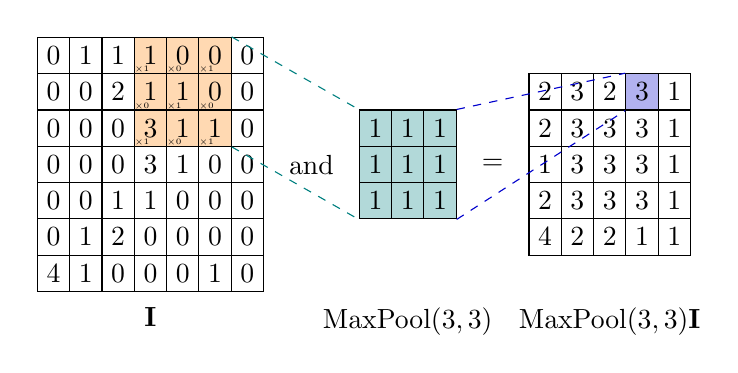
\begin{tikzpicture}[
    2d-arr/.style={matrix of nodes, row sep=-\pgflinewidth, column sep=-\pgflinewidth, nodes={draw}}
  ]

  \matrix (mtr) [2d-arr] {
  0 & 1 & 1 & |[fill=orange!30]| 1 & |[fill=orange!30]| 0 & |[fill=orange!30]| 0 & 0\\
  0 & 0 & 2 & |[fill=orange!30]| 1 & |[fill=orange!30]| 1 & |[fill=orange!30]| 0 & 0\\
  0 & 0 & 0 & |[fill=orange!30]| 3 & |[fill=orange!30]| 1 & |[fill=orange!30]| 1 & 0\\
  0 & 0 & 0 & 3 & 1 & 0 & 0\\
  0 & 0 & 1 & 1 & 0 & 0 & 0\\
  0 & 1 & 2 & 0 & 0 & 0 & 0\\
  4 & 1 & 0 & 0 & 0 & 1 & 0\\
  };

  \node[below=of mtr-5-4] {$\mathbf I$};

  \node[right=0.2em of mtr] (str) {and};

  \matrix (K) [2d-arr, right=0.2em of str, nodes={draw, fill=teal!30}] {
    1 & 1 & 1 \\
    1 & 1 & 1 \\
    1 & 1 & 1 \\
  };
  \node[below=of K-3-2] {MaxPool$(3,3)$};

  \node[right=0.2em of K] (eq) {$=$};

  \matrix (ret) [2d-arr, right=0.2em of eq] {
  2 & 3 & 2 & |[fill=blue!80!black!30]| 3 & 1\\
  2 & 3 & 3 & 3 & 1\\
  1 & 3 & 3 & 3 & 1\\
  2 & 3 & 3 & 3 & 1\\
  4 & 2 & 2 & 1 & 1\\
  };
  \node[below=of ret-4-3] {MaxPool$(3,3)\mathbf{I}$};

  \draw[dashed, teal] (mtr-1-6.north east) -- (K-1-1.north west);
  \draw[dashed, teal] (mtr-3-6.south east) -- (K-3-1.south west);

  \draw[dashed, blue!80!black] (K-1-3.north east) -- (ret-1-4.north west);
  \draw[dashed, blue!80!black] (K-3-3.south east) -- (ret-1-4.south west);

  \foreach \i in {1,2,3} {
      \foreach \j in {4,5,6} {
          \node[font=\tiny, scale=0.6, shift={(-1.2ex,-2ex)}] at (mtr-\i-\j) {$\times \pgfmathparse{int(mod(\i+\j,2))}\pgfmathresult$};
        }
    }

\end{tikzpicture}


\end{figure}
\end{frame}

\begin{frame}{Convolutional network architecture (CNN)}
Implemented in both libraries
\begin{itemize}
  \item input layer -- 794 signals ($28\times28$)
  \item 1st layer -- 10 filters 5x5, stride 1,1, tanh
  \item 2nd layer -- MaxPool 2x2, stride 2,2
  \item 3rd layer -- 20 filters 5x5, stride 1,1, tanh
  \item 4th layer -- MaxPool 2x2, stride 2,2
  \item 5th layer -- Dense, 50 neurons, tanh
  \item out layer -- 10 neurons softmax activation
\end{itemize}
\end{frame}

\begin{frame}{1D convolution}
We need to change dataset, one dimensional or time-series data is better in this case.
\begin{itemize}
\item We use \href{https://archive.ics.uci.edu/ml/datasets/human+activity+recognition+using+smartphones}{\color{blue}\underline{UCI HAR Dataset}}
\item It contain mobile sensors data, allow recision behaviour
\item walking, walking upstairs, walking downstairs, sitting, standing, laying
\item we use only global acceleration and as a total i.e $\text{a}=\sqrt{a_x^2+a_y^2+a_z^2}$
\begin{itemize}
  \item its not the best approach, but serves for this tutorial
  \item we should join three last classes as they should not be distinguished by acceleration
  \item code connected with data preparation is in file:\\ examples $\rightarrow$ Conv1D $\rightarrow$ read\_dataset.py
\end{itemize}
\item for PyTorch we prepare data for DataLoader
\item for Tensorflow we use OneHotEncoding
\end{itemize}
\end{frame}
\begin{frame}
Implemented in both libraries
\begin{itemize}
  \item input layer -- 128 signals (128 acc measurements)
  \item 1st layer -- Conv 1D, 64 filters 10x1, relu
  \item 2nd layer -- Conv 1D, 64 filters 10x1, relu
  \item 3rd layer -- Dropout (.15)
  \item 4th layer -- MaxPool1D 2, stride 2
  \item 5th layer -- Dense, 100 neurons, tanh
  \item out layer -- 6 neurons softmax activation
\end{itemize}
\end{frame}

\begin{frame}{Classification results analysis}
Confusion matrix is the easiest way to analyse the effects of our ML system

%\begin{tikzpicture}[scale=0.6]
%  \foreach \y [count=\n] in {
%    {1226, 0,    0,    0,    0,    0},
%    {3, 1070,    0,    0,    0,    0},
%    {0,    3,  983,    0,    0,    0},
%    {0,    0,    0,    0,  913,  373},
%    {0,    0,    0,    0, 1360,   14},
%    {1,    0,    0,    0,  134, 1272},
%    } {
%      % column labels
%      \ifnum\n<10
%        \node[minimum size=6mm] at (\n, 0) {\n};
%      \fi
%      % heatmap tiles
%      \foreach \x [count=\m] in \y {
%        \node[fill=yellow!\x!purple, minimum size=6mm, text=white] at (\m,-\n) {\x};
%      }
%    }
%
%  % row labels
%  \foreach \a [count=\i] in {a,b,c,d,e,f,g,h,i} {
%    \node[minimum size=6mm] at (0,-\i) {\a};
%  }
%\end{tikzpicture}
\begin{figure}
\centering
\hfill
\begin{subfigure}[b]{0.4\textwidth}
\resizebox{.9\textwidth}{!}{
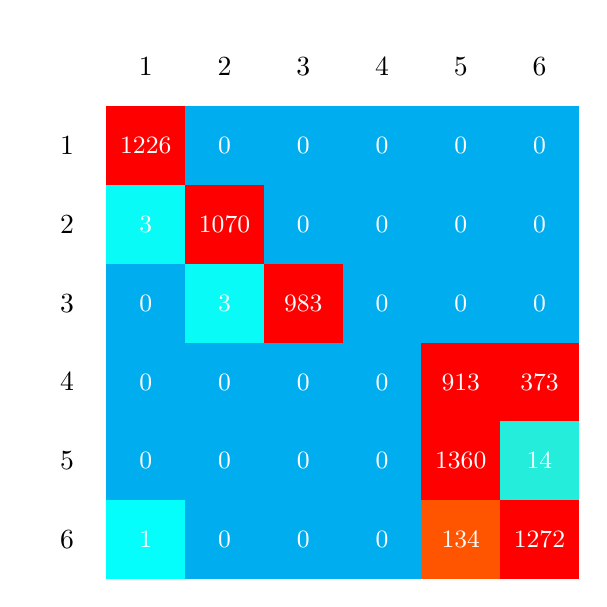
\begin{tikzpicture}
  \foreach \y [count=\n] in {
    {1226, 0,    0,    0,    0,    0},
    {3, 1070,    0,    0,    0,    0},
    {0,    3,  983,    0,    0,    0},
    {0,    0,    0,    0,  913,  373},
    {0,    0,    0,    0, 1360,   14},
    {1,    0,    0,    0,  134, 1272},
    } {
      % column labels
      \ifnum\n<7
        \node[minimum size=10mm] at (\n, 0) {\n};
      \fi
      % heatmap tiles
      \foreach \x [count=\m] in \y {
        \node[fill=orange!\x!cyan, minimum size=10mm,text=white] at (\m,-\n) {\small \x};
      }
    }

  % row labels
  \foreach \a [count=\i] in {1,2,3,4,5,6} {
    \node[minimum size=10mm] at (0,-\i) {\a};
  }
\end{tikzpicture}
}
\caption{Confusion matrix for train set, accuracy: $5911/7352 (80\%)$}
\end{subfigure}
\hfill
\begin{subfigure}[b]{0.4\textwidth}
\resizebox{.9\textwidth}{!}{
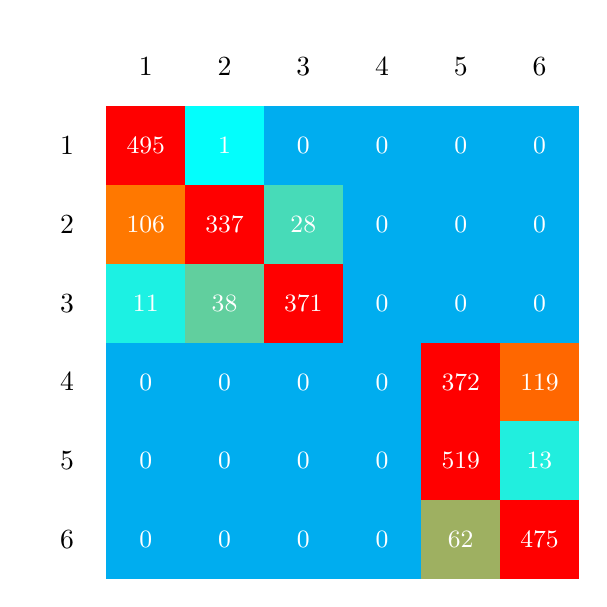
\begin{tikzpicture}
  \foreach \y [count=\n] in {
    {495,   1,  0,  0,  0,  0},
    {106, 337, 28,  0,  0,  0},
    {11,   38,371,  0,  0,  0},
    { 0,    0,  0,  0,372, 119},
    { 0,    0,  0,  0,519,  13},
    { 0,    0,  0,  0, 62, 475},
    } {
      % column labels
      \ifnum\n<7
        \node[minimum size=10mm] at (\n, 0) {\n};
      \fi
      % heatmap tiles
      \foreach \x [count=\m] in \y {
        \node[fill=orange!\x!cyan, minimum size=10mm,text=white] at (\m,-\n) {\small \x};
      }
    }

  % row labels
  \foreach \a [count=\i] in {1,2,3,4,5,6} {
    \node[minimum size=10mm] at (0,-\i) {\a};
  }
\end{tikzpicture}
}
\caption{Confusion matrix for test set, accuracy: $2197/2947 (75\%)$}
\end{subfigure}
\hfill
\end{figure}
\end{frame}

\begin{frame}{Advanced tasks}
This is shown only in PyTorch, but can be done (probaby) in Tensorflow.

Advanced analysis of the network, activations etc.
\begin{itemize}
\item We can always get weight and biases for our layers
\item We can watch ``live'' activations during feed forward pass
\begin{itemize}
\item Hook a layer,
\item Hook can be added to layer or layer after activation function is applied
\end{itemize}
\end{itemize}

\end{frame}

\end{document}
